
\documentclass{beamer}

\usepackage{algpseudocode, color, colortbl}

\usepackage{wrapfig}

\usetheme{Montpellier}
\usecolortheme{rose}

% page numbers, from
% https://tex.stackexchange.com/questions/137022/how-to-insert-page-number-in-beamer-navigation-symbols
\expandafter\def\expandafter\insertshorttitle\expandafter{%
  \insertshorttitle\hfill%
  \insertframenumber\,/\,\inserttotalframenumber}

\definecolor{Gray}{gray}{0.8}
\newcolumntype{g}{>{\columncolor{Gray}}c}

\newcommand{\stanza}{ \\~\ }

\title{11. Dynamic Programming Introduction}
\subtitle{CPSC 535}
\author{Kevin A. Wortman}
\institute{ 
\includegraphics[height=2cm]{csuf-logo-cmyk} }
\date{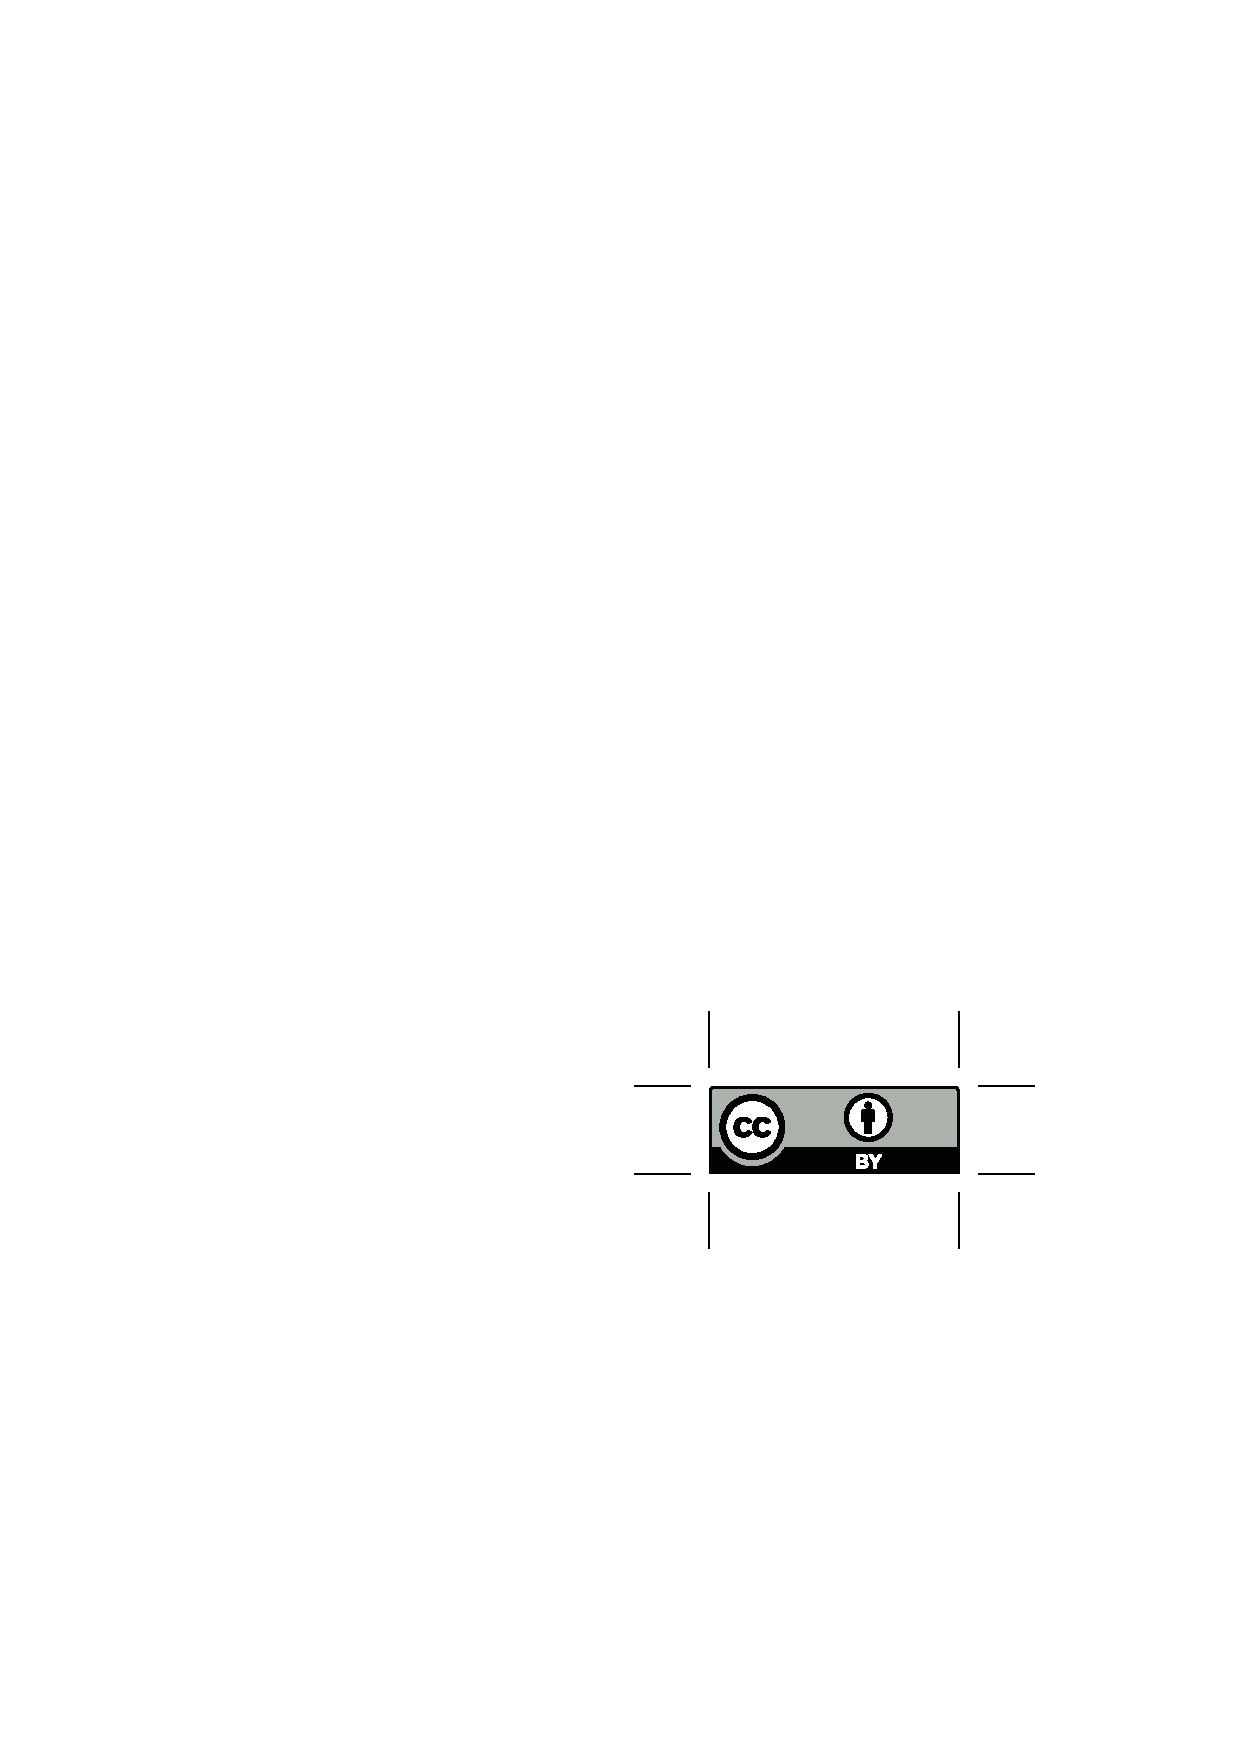
\includegraphics[height=14pt]{by} \\

{\tiny
This work is licensed under a
\href{http://creativecommons.org/licenses/by/4.0/}{Creative Commons Attribution 4.0 International License}.
}}

\begin{document}

\begin{frame}
  \titlepage
\end{frame}

\begin{frame} \frametitle{Dynamic Programming}
\begin{itemize}
  \item pattern for designing algorithms
  \item \emph{programming:}
  \begin{itemize}
    \item optimize subject to constraints
    \item (same as Linear Programming)
    \item \textbf{not} writing programs
  \end{itemize}
  \item \emph{dynamic:} curious buzzword
  \item specialized tool
  \begin{itemize}
    \item dynamic programming only applies to problems with \emph{overlapping subproblems}
    \item rare
    \item huge speedup over naive algorithms for such problems
  \end{itemize}
\end{itemize}
\end{frame}

\begin{frame} \frametitle{Big Ideas}
\begin{itemize}
  \item important algorithm design approach in its own right
  \item problem solving to view a problem in a different way
  \item \textbf{time-space trade-off}
  \begin{itemize}
    \item speedup costs space
  \end{itemize}
  \item \textbf{efficiency-complexity trade-off}
  \begin{itemize}
    \item top-down, bottom-up variants
    \item top-down is simpler to design and implement
    \item bottom-up has faster constant factors
  \end{itemize}
\end{itemize}
\end{frame}

\begin{frame} \frametitle{Optimization, Value, Solution}
\begin{itemize}
  \item dynamic programming usually applies to \textbf{optimization} problems
  \begin{itemize}
    \item correct output ``minimizes'' or ``maximizes'' something
  \end{itemize}
  \item \textbf{value:} quality of the solution
  \begin{itemize}
    \item quantity to minimize/maximize
  \end{itemize} 
  \item designing a dynamic programming algorithm to\dots
  \begin{itemize}
    \item ...calculate optimal \textbf{value} is simpler
    \item ...calculate optimal \textbf{solution} is more complicated
  \end{itemize}
  \item $\therefore$ some examples and exercises only involves \textbf{values}
  \item algo's for \textbf{solutions} are more practical but difficult
\end{itemize}
\end{frame}

\begin{frame} \frametitle{Example: Vertex Cover}
\emph{vertex cover problem} \\
\textbf{input:} an undirected graph $G=(V, E)$ \\
\textbf{output:} a vertex cover $C$ of minimum size
\begin{itemize}
  \item solution = a set of vertices $C$
  \item value = size of $C$
  \item optimal = minimize $|C|$ \stanza
\end{itemize}

\emph{vertex cover value problem} \\
\textbf{input:} an undirected graph $G=(V, E)$ \\
\textbf{output:} the minimum size of a vertex cover of $G$
\begin{itemize}
  \item note: output data type is an integer, not a set
\end{itemize}
\end{frame}

\begin{frame} \frametitle{Example: Bipartite Matching}
  \textbf{bipartite maximum matching problem} \\
  \emph{input:} an undirected bipartite graph $G=(V, E)$ with parts $V=L \cup R$ \\
  \emph{output:} a matching $M \subseteq E$ where the number of matched vertices
    is maximum    
  \begin{itemize}
    \item solution = a set of edges $M$
    \item value = size of $M$ \stanza
  \end{itemize}
  
  \textbf{bipartite maximum matching value problem} \\
  \emph{input:} an undirected bipartite graph $G=(V, E)$ with parts $V=L \cup R$ \\
  \emph{output:} the maximum number of edges in a matching of $G$ 
  \begin{itemize}
    \item note: output data type is an integer, not a set
  \end{itemize}
  \end{frame}
  
\begin{frame} \frametitle{Ties}
  \begin{itemize}
  \item we say \textbf{an} optimal solution
  \item not \textbf{the} optimal solution
  \item multiple solutions may have same value
  \item any of these are correct
  \item examples:
  \begin{itemize}
    \item vertex cover: ``a vertex cover $C$ of minimum size''
    \item bipartite matching: ``a matching $M \subseteq E$ where the number of matched vertices
    is maximum''
  \end{itemize}
  \item not worrying about ties simplifies dynamic programming algorithms
\end{itemize}
\end{frame}

\begin{frame} \frametitle{The Main Idea}
  \begin{itemize}
    \item dynamic programming works on a problem where\dots
    \begin{itemize}
      \item a solution has a \textbf{recursive structure}
      \item so we \emph{could} design a naive divide-and-conquer algorithm
      \item \textbf{but,} subproblems \textbf{overlap}
      \item so divide-and-conquer would do the same work repeatedly
      \item would be slow (often exponential time)
    \end{itemize}
    \item idea: store subproblem solutions in a \textbf{table} (array or hash dictionary)
    \item only solve subproblems not already in table
    \item $\therefore$ each subproblem is solved \textbf{only once}
    \item fast polynomial time, often $\Theta(n)$ or $\Theta(n^2)$
  \end{itemize}
\end{frame}

\begin{frame} \frametitle{Top-Down versus Bottom Up}
  \begin{itemize}
    \item two ways to write the pseudocode
    \item \textbf{top-down}
    \begin{itemize}
      \item improvement to divide-and-conquer pseudocode
      \item add a base case that checks for a solution in the table
      \item simple to derive from divide-and-conquer algorithm
      \item usually depends on a hash dictionary data structure, so expected time
    \end{itemize}
    \item \textbf{bottom-up}
    \begin{itemize}
      \item clean-sheet redesign
      \item nested loops explicitly solve problems in sorted order
      \item base case, larger subproblems, \dots, full problem
      \item store subproblems in array (not hash table)
      \item no recursion or hash table $\Rightarrow$ faster constant factors
    \end{itemize}
  \end{itemize}
\end{frame}

\begin{frame} \frametitle{Design Process}
\begin{enumerate}
  \item Identify the problem's \textbf{solution} and \textbf{value}, and note which is our \textbf{goal}.
  \item Derive a \textbf{recurrence} for an optimal value.
  \item Design a divide-and-conquer algorithm that computes an \textbf{optimal value}.
  \item Design a dynamic programming algorithm that computes an \textbf{optimal value}.
  \begin{enumerate}
    \item \textbf{top-down} alternative: add table base case (\textbf{memoization})
    \item \textbf{bottom-up} alternative: rewrite to use bottom-up loops instead of recursion
  \end{enumerate}
  \item (if goal is a solution algo.) Design a dynamic programming algorithm that computes an \textbf{optimal solution}.
\end{enumerate}
\end{frame}

\begin{frame} \frametitle{Rod Cutting Problem}
story:
\begin{itemize}
  \item have a rod of metal $n$ inches long
  \item can chop it into pieces of size $1, 2, \ldots, n$
  \item total length of all pieces $=n$
  \item market price of a $i$-inch piece is $p_i$
  \item market price of a 0-inch piece is 0
  \item goal: maximize total price of the pieces \stanza
\end{itemize}

\emph{rod cutting value problem} \\
\textbf{input:} an array of non-negative prices $P=\langle p_1, \ldots, p_n \rangle$ \\
\textbf{output:} the maximum total price that can be achieved by cutting an $n$-inch rod into pieces
  
\end{frame}

\begin{frame} \frametitle{Example with $n=4$}
\begin{center}
  \begin{tabular}{|l|l|l|l|l|} \hline
    $i$ & 1 & 2 & 3 & 4 \\ \hline
    $p_i$ & 3 & 7 & 8 & 11 \\ \hline
  \end{tabular}
\end{center}

Ways of cutting $\Box\Box\Box\Box$:
\begin{enumerate}
  \item $\Box\Box\Box\Box : p_4 = \$ 11$
  \item $\Box \mid \Box\Box\Box : p_1 + p_3 = \$3 + \$8 = \$11$
  \item $\Box\Box \mid \Box\Box : p_2 + p_2 = \$7 + \$7 = \$14$
  \item $\Box\Box\Box \mid \Box : p_3 + p_1 = \$8 + \$3 = \$11$
  \item $\Box \mid \Box \mid \Box\Box : p_1 + p_1 + p_2 = \$3 + \$3 + \$7 = \$13$
  \item $\Box \mid \Box\Box \mid \Box : p_1 + p_2 + p_1 = \$3 + \$7 + \$3 = \$13$
  \item $\Box\Box \mid \Box \mid \Box : p_2 + p_1 + p_1 = \$7 + \$3 + \$3 = \$13$
  \item $\Box \mid \Box \mid \Box \mid \Box : p_1 + p_1 + p_1 + p_1 = \$3 + \$3 + \$3 + \$3 = \$12$
\end{enumerate}

\end{frame}

\begin{frame} \frametitle{Greedy Fails}
\begin{itemize}
  \item greedy heuristics are \textbf{not correct} for this problem
  \item note that there is no requirement that prices $p_i$ obey ``common sense'' market dynamics
  \item e.g. it is allowed for $p_4 > p_5$
  \item example of an \textbf{incorrect} greedy heuristic: find length $i$ with highest unit price $p_i/i$, then make $\lceil n/i \rceil$ pieces of length $i$
  \item fails when the leftover $n-\lceil n/i \rceil$ inches could be used better
  \item Recall: the designer of a greedy algorithm has the burden of \textbf{proving} their heuristic is correct
  \item \textbf{Tip:} if you are told to design a dynamic programming algorithm, don't waste time with greedy algorithms
\end{itemize}
\end{frame}

\begin{frame} \frametitle{Rod Cutting Step 1}
\begin{enumerate}
  \item Identify the problem's \textbf{solution} and \textbf{value}, and note which is our \textbf{goal}.
  \stanza
\end{enumerate}
\emph{rod cutting value problem} \\
\textbf{input:} an array of non-negative prices $P=\langle p_1, \ldots, p_n \rangle$ \\
\textbf{output:} the maximum total price that can be achieved by cutting an $n$-inch rod into pieces
\begin{itemize}
  \item \textbf{solution:} list of piece lengths e.g. $\langle 2, 2 \rangle$
  \item \textbf{value:} total price e.g. $\$14$
  \item goal: \textbf{value}
\end{itemize}
\end{frame}

\begin{frame} \frametitle{Rod Cutting Step 2}
  \begin{enumerate}
    \setcounter{enumi}{1}
    \item Derive a \textbf{recurrence} for an optimal value.
    \stanza
  \end{enumerate}

  \begin{itemize}
    \item define $r_i = $ the maximum total price starting from $i$ inches
    \item base case: $r_0 = 0$
    \item general case:
    \begin{itemize}
      \item \textbf{think} divide-and-conquer; define $r_i$ in terms of $r_{<i}$
      \item make the problem \textbf{one piece} smaller
      \item try to make one cut, then recursively use the remaining inches
      \item try every option and keep the optimal one
      \[ r_i = \max_{1 \leq i \leq n} (p_i + r_{n-i}) \]
    \end{itemize}
  \end{itemize}
\end{frame}
  
\begin{frame} \frametitle{Rod Cutting Step 3}
  \begin{enumerate}
    \setcounter{enumi}{2}
    \item Design a divide-and-conquer algorithm that computes an \textbf{optimal value}.
    \stanza
  \end{enumerate}

  \begin{algorithmic}[1]
    \Function{CUT-ROD-DC}{P, n}
    \If{ n ==0 }
      \State \Return{ 0 }
    \EndIf
    \State $q = -\infty$
    \For {$i$ from 1 to $n$}
      \State $q = \max(q, P[i] + \text{CUT-ROD-DC(P, n-i)})$
    \EndFor
    \State \Return{$q$}
    \EndFunction
  \end{algorithmic}
\end{frame}

\begin{frame} \frametitle{Sidebar: Analysis of CUT-ROD-DC}
\begin{itemize}
  \item CUT-ROD-DC corresponds directly to the $r_i$ defition
  \item \textbf{but} it is very slow
  \item fundamental problem: CUT-ROD-DC calls itself many times
  \begin{itemize}
    \item each iteration of the \textbf{for} loop is a recursive call
    \item each of those has a \textbf{for} loop with recursive calls\ldots
  \end{itemize}
  \item recall: fast divide-and-conquer algorithms usually call themselves 1--2 times
  \item \emph{Claim:} The time complexity of CUT-ROD-DC is $O(2^{n-1}).$
  \item dynamic programming will circumvent all this recursion
\end{itemize}
\end{frame}

\begin{frame} \frametitle{Rod Cutting Step 4.a}
  \begin{enumerate}
    \setcounter{enumi}{3}
    \item Design a dynamic programming algorithm that computes an \textbf{optimal value}.
    \begin{enumerate}
      \item \textbf{top-down} alternative: add table base case (\textbf{memoization})
      \stanza
    \end{enumerate}
\end{enumerate}

\begin{itemize}
  \item \textbf{memoization:} use a hash dictionary to make a ``memo'' of pre-calculated solutions
  \item use $i$ as key in table $T$ (same API as hash tables in deck 4)
  \item after we compute an $r_i,$ set $r_i.key = i$ and insert $r_i$ into $T$
  \item if $T$ does not contain key $i,$ then we haven't computed $r_i$ yet
  \item need two functions
  \begin{itemize}
    \item public non-recursive function to create $T$ and start recursion
    \item private recursive function that expects $T$ to exist
  \end{itemize}
\end{itemize}
\end{frame}

\begin{frame} \frametitle{Rod Cutting Step 4.a}
  {\scriptsize
  \begin{algorithmic}[1]
    \Function{CUT-ROD-MEMOIZED}{P, n}
    \State HASH-TABLE-CREATE($T$)
    \State \Return{CUT-ROD-MEMO-REC($T, P, n$)}
    \EndFunction
    \Function{CUT-ROD-MEMO-REC}{$T, P, n$}
    \State $q = $ HASH-TABLE-SEARCH($T, n$)
    \If{ $q \ne$ NIL }
      \State \Return{ $q$ }
    \EndIf
    \If{ n == 0 }
      \State $q=0$
    \Else
      \State $q=-\infty$
      \For {$i$ from 1 to $n$}
        \State $q = \max(q, P[i] + \text{CUT-ROD-MEMO-REC(T, P, n - i)})$
      \EndFor
    \EndIf
    \State $q.key = n$
    \State HASH-TABLE-INSERT($q$)
    \State \Return{$q$}
    \EndFunction
  \end{algorithmic}
  }
\end{frame}

\begin{frame} \frametitle{Rod Cutting Step 4.b}
  \begin{enumerate}
    \setcounter{enumi}{3}
    \item Design a dynamic programming algorithm that computes an \textbf{optimal value}.
    \begin{enumerate}
      \item \textbf{top-down} alternative: add table base case (\textbf{memoization})
      \item \textbf{bottom-up} alternative: rewrite to use bottom-up loops instead of recursion
      \stanza
    \end{enumerate}
\end{enumerate}

\begin{itemize}
  \item observe: in CUT-ROD-MEMOIZED, keys are inserted into $T$ in order $0, 1, \ldots, n$
  \item \textbf{bottom-up:} write an explicit \textbf{for} loop that computes and stores every general case $r_i$ in order $r_1, \ldots, r_n$
  \item base case is computed and stored before the loop
  \item convenient to use an array instead of hash table
  \item define $R[i] = r_i$
  \item no more recursion, just loops
\end{itemize}
\end{frame}

\begin{frame} \frametitle{Rod Cutting Step 4.b}
  {\small
  \begin{algorithmic}[1]
    \Function{CUT-ROD-BU}{P[1..n]}
    \State Create array $R[0..n]$
    \State $R[0] = 0$
    \For{$j$ from 1 to $n$}
      \State $q=-\infty$
      \For{$i$ from 1 to $n$}
        \State{$q = \max(q, P[i] + R[j-i])$}
      \EndFor
      \State $R[j] = q$
    \EndFor
    \State \Return $R[n]$
    \EndFunction
  \end{algorithmic}
  }
\end{frame}

\begin{frame} \frametitle{Bottom-Up Analysis}
  \begin{itemize}
    \item CUT-ROD-BU is clearly $\Theta(n^2)$ time
    \item (Note: easy analysis)
  \end{itemize}
\end{frame}

\begin{frame} \frametitle{Top-Down Analysis}
    \begin{itemize}
      \item trickier analysis
      \item observe: hash \textbf{if} statement guarantees that each subproblem is solved exactly once
      \item solving subproblem $i,$ not counting recursion: $\Theta(i)$ time due to \textbf{for} loop
      \item total of all subproblems is $\sum_{i=1}^n i \in \Theta(n^2)$
      \item hash operations add ``expected'' qualifier
      \item $\therefore$ CUT-ROD-MEMOIZED takes $\Theta(n^2)$ expected time
      \item with effort we could replace the hash table with an array for $\Theta(n^2)$ worst-case time
      \item CUT-ROD-MEMOIZED has worse constant factors due to the overhead of recursive function calls
    \end{itemize}
\end{frame}

\begin{frame} \frametitle{Trade-Offs}
\begin{center}
  \begin{tabular}{llll}
    \textbf{Factor} & \textbf{Naive} & \textbf{TDDP} & \textbf{BUDP} \\ \hline
    Ease of design & easiest & difficult & very difficult \\
    Ease of analysis & medium & difficult & easy \\
    Time efficiency & $O(2^{n-1})$ & $\Theta(n^2)$ exp. & $\Theta(n^2)$ w/ fast const. \\
    Space overhead & n/a & $O(n)$ hashtable & $O(n)$ array \\
  \end{tabular}
\end{center}

\begin{itemize}
  \item according to principles, \textbf{bottom up dynamic programming} is superior
  \item but top-down dynamic programming is a close second
\end{itemize}
\end{frame}

\begin{frame} \frametitle{Subproblem Graphs}
\begin{itemize}
  \item solutions have a recursive structure
        \[ r_i = \max_{1 \leq i \leq n} (p_i + r_{n-i}) \]
  \item a general-case solution depends on other solution(s)
  \item algorithm must compute solutions in an order that satisfies dependencies
  \item memoization automates this, with overhead
  \item bottom-up loops must be designed carefully to iterate in satisfactory order
  \item visualize dependencies in a \textbf{subproblem graph}
\end{itemize}
\end{frame}

\begin{frame} \frametitle{Subproblem Graphs}
  \begin{center}
    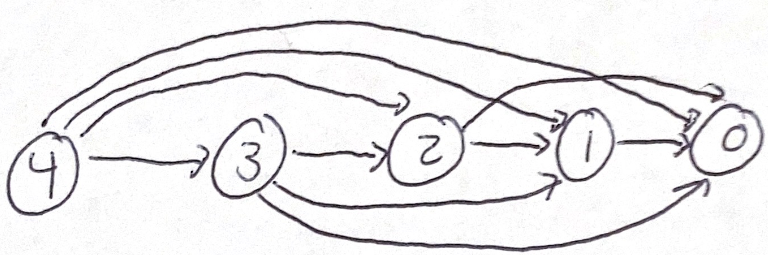
\includegraphics[height=.8in]{subproblem_dependencies.png}
  \end{center}
  \begin{itemize}
  \item vertex $i$ = subproblem $i$
  \item directed edge $(i, j)$ = computing $i$ requires solution to $j$
  \item subproblem $i$ must wait until all outgoing neighbors have been computed
  \item top-down manages with hashtable
  \item bottom up manages with loop iteration order
  \end{itemize}
\end{frame}

\begin{frame} \frametitle{Rod Cutting Step 5}
  \begin{enumerate}
    \setcounter{enumi}{4}
    \item (if goal is a solution algo.) Design a dynamic programming algorithm that computes an \textbf{optimal solution}.
    \stanza
  \end{enumerate}

  
  \emph{rod cutting value problem} \\
  \textbf{input:} an array of non-negative prices $P=\langle p_1, \ldots, p_n \rangle$ \\
  \textbf{output:} the maximum total price that can be achieved by cutting an $n$-inch rod into pieces
  \stanza

  \emph{rod cutting problem} \\
  \textbf{input:} an array of non-negative prices $P=\langle p_1, \ldots, p_n \rangle$ \\
  \textbf{output:} the list of cut-lengths of maximum total price for an $n$-inch rod

\end{frame}

\begin{frame} \frametitle{Storing All Subproblem Solutions Is Expensive}
  \begin{itemize}
    \item solution to rod cutting problem: a list of cut-lengths; $O(n)$ space each
    \item our algorithms compute $n+1$ solutions
    \item storing all subproblem solutions would takes $O((n+1)\times n) = O(n^2)$ space, \textbf{expensive}
    \item instead, store only $O(n)$ information
  \end{itemize}
\end{frame}

\begin{frame} \frametitle{Backtracking}
  \begin{itemize}
    \item algorithm computes optimal value, and \textbf{logs (records) how it made each decision}
    \item after all optimal values have been computed, follow a ``trail'' to create solution object
    \item trail ends at the optimal solution
    \item each log entry says how to go one step backwards
    \item follow them until we get to the start (a base case)
    \item traverses solution in backwards order; reverse it if order matters
    \item backtracking is usually only $O(n)$ time, and $O(n)$ space overhead
  \end{itemize}
\end{frame}

\begin{frame} \frametitle{Rod Cutting Step 5}
  \begin{enumerate}
    \setcounter{enumi}{4}
    \item (if goal is a solution algo.) Design a dynamic programming algorithm that computes an \textbf{optimal solution}.
  \end{enumerate}

  \begin{itemize}
    \item bottom-up algo. makes optimal choices with
      \[ q = \max(q, P[i] + R[j-i]) \]
      step
    \item i.e. it chooses how many inches to cut right now
    \item \textbf{log} these choices in another array
    \item recall $R[j] = $ maximum total price starting from $j$ inches
    \item define $S[j] = $ size of the first optimal cut starting from $j$ inches
    \item need to update pseudocode to
    \begin{itemize}
      \item create $S$
      \item update $S$ inside the loops
      \item at the end, backtrack $S$ to compute a list of lengths
    \end{itemize}
  \end{itemize}
\end{frame}

\begin{frame} \frametitle{Rod Cutting Step 5 -- Pseudocode}
  {\tiny
  \begin{algorithmic}[1]
    \Function{CUT-ROD-SOLUTION}{P[1..n]}
    \State Create arrays $R[0..n]$ and $S[0..n]$
    \State $R[0] = 0$
    \For{$j$ from 1 to $n$}
      \State $q=-\infty$
      \For{$i$ from 1 to $n$}
        \If{ $q < (P[i] + R[j-1])$ }
          \State{$q = P[i] + R[j-i]$}
          \State{$S[j] = i$}
        \EndIf
      \EndFor
      \State $R[j] = q$
    \EndFor
    \State soln = empty list
    \State $j = n$
    \While { $j > 0$ }
      \State soln.add($S[j]$)
      \State $j = j - S[j]$
    \EndWhile
    \State reverse soln
    \State \Return{soln}
    \EndFunction
  \end{algorithmic}
  }
\end{frame}

\begin{frame}{Analysis}
  \begin{itemize}
    \item CUT-ROD-SOLUTION solves the \emph{rod cutting problem}
    \begin{itemize}
      \item it returns a list of cut-lengths, not a price
    \end{itemize}
    \item analysis is actually straightforward
    \item time efficiency:
    \begin{itemize}
      \item nested \textbf{for} loops: $\Theta(n^2)$
      \item backtracking: \textbf{while} loop iterates at most $n$ times $\Rightarrow \Theta(n)$ time
      \item reverse soln: $\Theta(n)$
      \item total $\Theta(n^2+n+n)=\Theta(n^2)$ time
    \end{itemize}
    \item space efficiency: $R$ and $S$ take $\Theta(n+n)=\Theta(n)$ space
    \item (same as the step-4 algorithms)
  \end{itemize}
\end{frame}

\end{document}
